% Capítulo 6 — Conclusões (orçamento: ~8 pp)
% Fechar sem inflacionar. As limitações são ditas em voz alta, incluindo a que fica em aberto.

\chapter{Conclusões}
\label{cap:conclusoes}

\section{Síntese do trabalho}
\label{sec:con_feito}

Existe um sistema a funcionar, e não uma demonstração. O InvestiGator vigia doze empresas, corre de
forma contínua, e envia alertas explicados a um canal público, com uma página web onde o que
foi enviado pode ser consultado depois.

E existe uma avaliação de cada uma das quatro técnicas, com os resultados reportados como se
revelaram. Três foram medidas \emph{contra alternativas mais simples}, que é o desenho que permite
dizer que não. A quarta, a decomposição, não podia sê-lo, porque não existe uma resposta certa
contra a qual comparar uma repartição: dela mede-se o que é mensurável, que é a qualidade do
ajuste, e a Secção~\ref{sec:av_decomposicao} explica porquê. É esta parte que dá ao trabalho o
carácter de dissertação e não o de projeto.

Vale a pena dizer também onde está a engenharia, porque a resposta não é o tamanho do modelo.
Este trabalho treina um só, e é pequeno. O que foi preciso construir para que o número dele, e
a conclusão negativa que ele sustenta, sejam de confiança está reunido na
Secção~\ref{sec:sis_ciclo_vida}: o conjunto de dados rotulado, a separação temporal imposta por
um teste, a calibração com o seu enviesamento declarado, os artefactos versionados, a garantia
de que o modelo implantado é o modelo avaliado, e o ciclo que observa o sistema depois de estar
a correr. É aí, e não no modelo, que está o trabalho.

\section{As respostas às perguntas de investigação}
\label{sec:con_qi}

A Figura~\ref{fig:con_scorecard} responde às três de uma vez, e o resto desta secção diz o que
cada resposta permite e não permite afirmar.

\begin{figure}[ht]
\centering
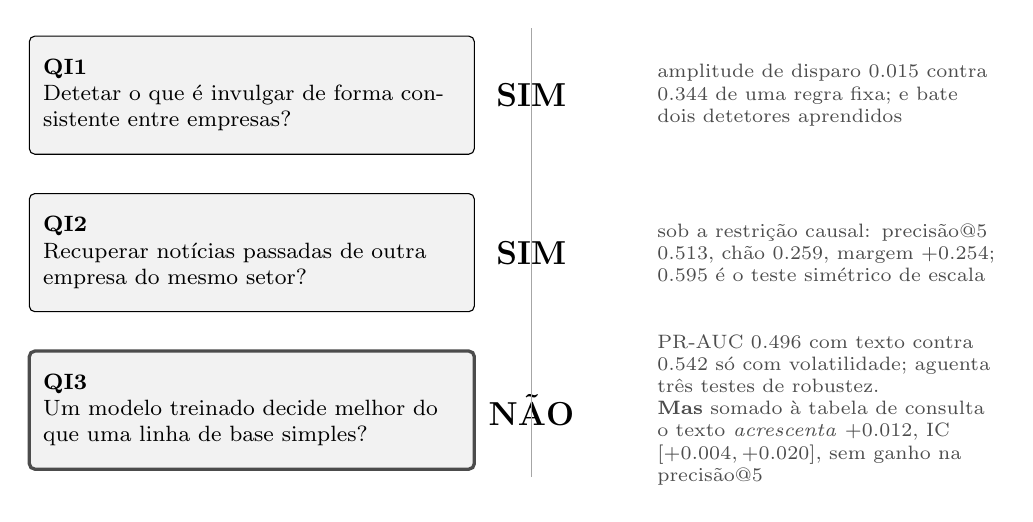
\begin{tikzpicture}[font=\footnotesize,
  cx/.style={draw, rounded corners=2pt, align=left, inner sep=5pt, text width=5.3cm,
             minimum height=1.5cm},
  sim/.style={cx, fill=black!5},
  nao/.style={cx, fill=black!5, draw=black!70, very thick},
  ver/.style={font=\bfseries\large, align=center},
  num/.style={align=left, text width=4.3cm, font=\scriptsize, text=black!70},
]
  \node[sim] (q1) at (0,0)      {\textbf{QI1} \\ Detetar o que é invulgar de forma consistente
                                  entre empresas?};
  \node[ver] at (3.55,0)        {SIM};
  \node[num] at (7.3,0)         {amplitude de disparo $0.015$ contra $0.344$ de uma regra fixa;
                                  e bate dois detetores aprendidos};

  \node[sim] (q2) at (0,-2.0)   {\textbf{QI2} \\ Recuperar notícias passadas de outra empresa
                                  do mesmo setor?};
  \node[ver] at (3.55,-2.0)     {SIM};
  \node[num] at (7.3,-2.0)      {sob a restrição causal: precisão@5 $0.513$, chão $0.259$,
                                  margem $+0.254$; $0.595$ é o teste simétrico de escala};

  \node[nao] (q3) at (0,-4.0)   {\textbf{QI3} \\ Um modelo treinado decide melhor do que uma
                                  linha de base simples?};
  \node[ver] at (3.55,-4.0)     {NÃO};
  \node[num] at (7.3,-4.0)      {PR-AUC $0.496$ com texto contra $0.542$ só com volatilidade;
                                  aguenta três testes de robustez.\\
                                  \textbf{Mas} somado à tabela de consulta o texto
                                  \emph{acrescenta} $+0.012$, IC $[+0.004, +0.020]$,
                                  sem ganho na precisão@5};

  \draw[black!35] (3.55,-4.85) -- (3.55,0.85);
\end{tikzpicture}
\caption[As três perguntas e as suas respostas]{O resultado do trabalho numa figura, com a resposta
negativa apresentada com o mesmo destaque das outras duas. A terceira linha é a que mais custou a
escrever e é a que dá crédito às outras: um trabalho que só reporta o que correu bem não permite
saber se as duas primeiras respostas foram medidas ou desejadas.}
\label{fig:con_scorecard}
\end{figure}

\paragraph{QI1, deteção. Sim.}
Um \emph{z}-score deslizante deteta movimentos invulgares de forma muito mais consistente entre
empresas do que uma regra fixa: uma amplitude de disparo de $0.015$ contra $0.344$, mais de vinte
vezes melhor. E, sujeito a uma comparação justa, ganha também a dois métodos de aprendizagem
desenhados para esta tarefa \autocite{liu2008isolation, breunig2000lof}.

Este resultado é menos surpreendente do que parece à primeira vista, e a literatura ajuda a
perceber porquê. Os dois métodos aprendidos decidem o que é invulgar pela geometria dos dados
\autocite{liu2008isolation, breunig2000lof}, um isolando o ponto raro e o outro comparando
densidades, e foram desenhados para situações com muitas variáveis
a interagir; aqui há uma série de retornos por empresa, e a estrutura que interessa é temporal, não
geométrica. A janela
deslizante capta diretamente o \emph{agrupamento de volatilidade}, a propriedade que os modelos
\gls{ARCH} e \gls{GARCH} formalizam \autocite{engle1982arch, bollerslev1986garch} sobre séries de inflação e que a
Secção~\ref{sec:av_qi1} mede nos retornos analisados aqui, ao passo que um detetor treinado sobre o conjunto
todo tem de aprender essa estrutura a partir dos dados. Quando a suposição de um método simples
coincide com a estrutura real do problema, é difícil batê-lo.

\paragraph{QI2, precedentes. Sim.}
A recuperação por significado encontra notícias passadas de outra empresa do mesmo setor sob a
restrição que o produto realmente tem: precisão@5 de $0.513$, chão $0.259$ e margem $+0.254$. O
teste simétrico sobre o corpus completo dá $0.595$, mas permite candidatos posteriores e serve como
teste de escala, não como número da tarefa causal. No corpus recente, o método supera sobreposição
de palavras, acaso uniforme e recência ($0.514$ contra $0.346$, $0.240$ e $0.126$). A linha de base
lexical medida é a mais simples da sua família, e não uma função de ordenação afinada, o que
delimita o alcance da afirmação.

\textbf{E o número agregado não é a forma certa de dizer isto}, pela razão que a
Secção~\ref{sec:av_qi2} desmonta: quase metade das consultas vem de um só setor, e existe uma
estratégia sem modelo nenhum, \emph{devolver sempre notícias desse setor}, que obtém $0.467$ sem
olhar para a pergunta. Contra ela a margem do método é de $+0.047$, e não de $+0.274$. Essa
estratégia é inútil como produto, porque acerta em tudo num setor e em nada nos outros quatro, mas
a sua existência mostra que o agregado mede em parte a composição do corpus. A afirmação que fica
é a de dentro de cada setor, onde ela não se aplica: a recuperação semântica supera a taxa-base
\textbf{nos cinco}, e o ganho é maior onde o corpus é mais fino.

Com uma segunda ressalva, que ficou clara ao medir: a semelhança capta o \textbf{tema}, não a
\textbf{direção}.

Essa ressalva é coerente com o que se esperaria, e não é apenas um defeito da implementação. A
hipótese dos mercados eficientes na sua forma semiforte \autocite{fama1970efficient} diz que a
informação pública já está refletida no preço; se assim for, a direção de um movimento futuro não
deveria ser recuperável a partir do tema de uma notícia pública. Convém ser cuidadoso com o estatuto
disto: trata-se de uma hipótese e não de uma lei, e o próprio autor sublinha que os seus testes são
sempre conjuntos, da eficiência e de um modelo de formação de preços ao mesmo tempo. Este trabalho
não a testa nem se apoia nela para concluir seja o que for. Serve apenas para dizer que o resultado
medido não é anómalo, e é uma das razões pelas quais o produto apresenta os precedentes como
observações do passado e nunca como indicação do que vem a seguir.

\paragraph{QI3, triagem. Não.}
Nenhum modelo que lê o texto do título bateu uma linha de base que usa apenas volatilidade
($0.496$ contra $0.542$). O resultado sobreviveu a um re-teste em condições favoráveis ao texto, a
uma reamostragem por grupos, e a nove definições diferentes do rótulo.

A resposta é negativa e é preciso dizê-la com a precisão que ela ganhou no fim do trabalho. Todas
essas comparações põem as variantes \emph{lado a lado}, e respondem por isso a \emph{qual é
melhor}. A pergunta que faltava era outra, e mais útil para quem constrói um sistema:
\emph{o texto acrescenta ao que já se sabe?} Medida por cima da tabela de consulta por empresa,
que a Secção~\ref{sec:av_ablacao} mostra conter tudo o que o modelo sabe da empresa e nada da
notícia, a resposta é \textbf{sim}, com $+0.012$ de PR-AUC e um intervalo $[+0.004, +0.020]$ que
exclui zero.
É detetável neste protocolo, pequeno, e é a única vez neste trabalho em que uma representação de texto mostra valor
mensurável.

Três medições impedem que isso reabra o veredicto, e estão na Secção~\ref{sec:av_acrescimo}: a
diferença para a volatilidade sozinha continua a ter um intervalo que contém zero; a precisão
dentro do orçamento não muda uma casa decimal, ou seja o ganho não sobrevive à métrica que
descreve o produto; e a capacidade de separar dois dias da mesma empresa continua ao nível do
acaso. O que isto acrescenta ao ``não'' não é uma ressalva, é uma \textbf{localização}: a
informação que o texto traz distingue empresas e períodos, e o produto precisava que distinguisse
notícias. É essa a diferença entre um resultado negativo e um resultado negativo compreendido, e é
ela que aponta o trabalho seguinte na Secção~\ref{sec:con_futuro}.

Esta última resposta é negativa e é a que eu levo mais a sério. Escrevi o critério de sucesso antes
de correr a experiência, e o resultado foi ao contrário do que eu esperava. Reportá-lo tal como
caiu era a única opção compatível com o resto do trabalho.

Existe uma linha de investigação considerável que usa texto para antecipar movimentos de preço
\autocite{xing2018nlffsurvey, ding2015deep}, e seria cómodo apresentar este resultado como se a
contradissesse. Não a contradiz, e convém ser preciso sobre porquê, incluindo num ponto em que a
diferença é menor do que eu gostaria. \textcite{ding2015deep} trabalham também sobre \emph{títulos},
e não sobre o corpo dos artigos, pelo que a diferença não está aí. Está no que se faz com eles:
extraem estruturas de acontecimento, do tipo ator, ação e objeto, e treinam uma rede para prever a
direção do movimento, ao passo que aqui se compara o título inteiro por semelhança e se recusa
prever direção. Os corpora e os horizontes de avaliação também diferem.

O que aqui se mostra é, portanto, mais estreito do que uma refutação, e é essa a afirmação que faço:
\textbf{sob esta restrição de dados e com esta família de métodos}, ou seja títulos de fontes
gratuitas comparados por semelhança de frase, o sinal textual não acrescenta ao que a volatilidade
recente já dizia. É um resultado sobre um regime de recursos e uma escolha de representação, e não
sobre a linguagem.

\section{Objetivos alcançados}
\label{sec:con_objetivos}

Dos quatro objetivos da Secção~\ref{sec:intro_objetivos}, \textbf{três estão cumpridos e um está
cumprido por metade}.

\begin{enumerate}
  \item \emph{Construir o sistema completo.} Cumprido. Os dois gatilhos funcionam de ponta a ponta,
        em produção.
  \item \emph{Avaliar cada componente contra linhas de base transparentes.} Cumprido para os três
        componentes em que foi definido um referente, e num deles mais do que o prometido: o detetor
        foi comparado não só com uma regra fixa mas também com dois métodos aprendidos. Para a
        decomposição não há verdade de terreno que permita medir exatidão; usaram-se ajuste e
        estabilidade, mas ficaram por comparar, por exemplo, mercado apenas contra mercado mais
        setor e betas brutos contra encolhidos. O que foi medido está na
        Secção~\ref{sec:av_decomposicao}.
  \item \emph{Garantir que as explicações são fiéis.} \textbf{Cumprido por metade.} A fidelidade
        está garantida por construção: o texto é montado a partir dos objetos calculados, e não
        pode divergir deles. Mas a \emph{utilidade} para uma pessoa real não foi medida, porque não
        se chegou a fazer um estudo com utilizadores. Não se afirma nada sobre ela.
  \item \emph{Reportar os resultados tal como se revelarem.} Cumprido, e a prova é o resultado
        negativo da QI3 estar no documento com o mesmo destaque dos outros dois.
\end{enumerate}

\section{Limitações}
\label{sec:con_limitacoes}

Ditas em voz alta, por ordem de importância. A Figura~\ref{fig:con_limites} resume as cinco
principais e o que cada uma pediria para ser fechada.

\begin{figure}[ht]
\centering
\begin{tikzpicture}[font=\footnotesize, >={Stealth[length=2mm]},
  lim/.style={draw, rounded corners=2pt, align=left, text width=4.9cm, inner sep=4pt,
              minimum height=0.95cm, fill=black!5},
  fut/.style={draw, rounded corners=2pt, align=left, text width=4.4cm, inner sep=4pt,
              minimum height=0.95cm, fill=white},
  cst/.style={align=center, text width=1.9cm, text=black!60, font=\scriptsize},
]
  \node[font=\bfseries\scriptsize, text=black!70] at (0,1.15)  {limitação, e está medida};
  \node[font=\bfseries\scriptsize, text=black!70] at (6.6,1.15) {o que a fecha};
  \node[font=\bfseries\scriptsize, text=black!70] at (11.1,1.15) {o que custa};
  % ⚠️ As variaveis do \foreach nunca podem chamar-se \c \t \l \i \o: sao comandos do LaTeX e a
  % substituicao acontece tambem DENTRO das palavras.
  \foreach \xn/\xlim/\xfut/\xcus in {%
    0/{Nenhuma avaliação com pessoas}/{Correr o estudo desenhado: 6 a 10 participantes}/{tempo de calendário},%
    1/{Os rótulos são aproximações}/{Anotar uma amostra com julgamento humano}/{tempo de calendário},%
    2/{O alerta afirma mais evidência do que tem}/{Medir o impacto por notícia, e não por dia}/{dados e anotação},%
    3/{Só se lê o título, e não o corpo}/{Recolher e representar o texto integral}/{dados novos},%
    4/{A deriva é medida e não corrigida}/{Re-treinar com o que se observa em produção}/{baixo}%
  } {
    \node[lim] (L\xn) at (0,-\xn*1.12) {\xlim};
    \node[fut] (F\xn) at (6.6,-\xn*1.12) {\xfut};
    \node[cst] at (11.1,-\xn*1.12) {\xcus};
    \draw[->, thick, black!40] (L\xn) -- (F\xn);
  }
\end{tikzpicture}
\caption[As limitações e o que as fecha]{Cada limitação desta secção foi \textbf{medida}, e não
apenas afirmada. A coluna do meio é o trabalho que cada uma pede, e a da direita é a razão pela
qual ainda não foi feito. As duas primeiras partilham o mesmo obstáculo, que é o único deste
trabalho com relógio de calendário: sem julgamento humano sobre uma amostra, nem a utilidade das
explicações nem a qualidade dos rótulos podem deixar de ser aproximações.}
\label{fig:con_limites}
\end{figure}

\paragraph{Não há estudo com utilizadores.}
É a lacuna maior e a mais fácil de nomear. Todo o sistema é construído à volta da ideia de que uma
explicação ajuda um não-especialista a decidir melhor, e essa ideia \textbf{não foi testada com
pessoas}. O desenho do estudo existe, com participantes, tarefas e critérios definidos, mas não foi
corrido a tempo. Enquanto isso não acontecer, a metade ``útil'' do terceiro objetivo fica sem resposta, e é assim
que está escrito.

A literatura é explícita quanto ao peso desta falta. Afirmações de interpretabilidade exigem
avaliação e não basta declará-las \autocite{doshivelez2017rigorous}, e o motivo não é
formalismo: o efeito de uma explicação sobre uma pessoa não é dedutível da sua construção. O que se
sabe é que a confiança pode falhar nos \emph{dois} sentidos, ignorando um aviso correto ou aceitando
um errado \autocite{lee2004trust}, e que a simples presença de uma explicação chega para aumentar a
aceitação de respostas erradas \autocite{bansal2021whole}. Este sistema é construído para tornar a
confiança apropriada, mostrando a evidência em vez de emitir um veredicto, mas \emph{que o consiga} é
uma hipótese por verificar e não um resultado. Note-se, aliás, que sem estudo com pessoas eu não
consigo distinguir os dois modos de falha: um alerta ignorado e um alerta indevidamente acreditado
são, para os meus registos, exatamente a mesma ausência de dados.

\paragraph{Os alertas ainda não estão bem calibrados, e sei disso a usar.}
Esta é a limitação que mais me incomoda, precisamente porque a noto como utilizador e não nos
números. Recebo no telemóvel, por outras vias, notícias sobre estas empresas que o sistema não
assinalou. E há dias em que uma ação sobe bastante e não gera alerta nenhum.

Parte disto está medido, e o número está na Secção~\ref{sec:av_pontaaponta}: sobre um ano de
notícias captadas, existia pelo menos uma notícia relevante em $88.5\%$ dos dias que o detetor
considerou invulgares. Os restantes $11.5\%$ são dias em que
\textbf{nenhuma alteração ao código ajuda}: se a fonte gratuita não associou nenhuma notícia à
empresa, ela nunca entra no funil. E a cobertura é muito desigual: a empresa pior coberta fica-se
pelos $50\%$.

Mas esse número é um \textbf{limite superior}, e a distinção importa: ele pergunta se existia
\emph{uma} notícia, não se chegou \emph{a certa}. Saber isso exigiria julgamento humano dia a dia, e
é trabalho por fazer.

\paragraph{O alerta afirma mais evidência do que tem.}
Quando mostra três precedentes e diz que os três se moveram na mesma direção, está a apresentar isso
como concordância entre três casos. Só que o impacto é medido por \emph{(empresa, dia)}: três
títulos da mesma empresa no mesmo dia partilham o mesmo valor por construção. Medido sobre os
$247$ alertas já entregues com precedentes, em $36.8\%$ deles os casos assentam em menos dias
distintos do que casos mostrados, e em $11.3\%$ são todos do mesmo dia. Não afeta nenhum número do
Capítulo~\ref{cap:avaliacao}; afeta o que o produto diz ao utilizador.

O alerta passou a contar dias e não títulos, o que torna a afirmação verdadeira. Mas a causa de
fundo continua lá: o impacto \emph{é} medido por dia, portanto duas notícias do mesmo dia nunca
poderão ser duas observações independentes, por mais que se conte bem. Medir impacto por notícia
exigiria, à escala do corpus, histórico intradiário fiável, horas de publicação exatas e uma regra
de atribuição capaz de separar notícias concorrentes. Esse conjunto não foi recolhido nem validado
neste trabalho; a existência de uma cotação intradiária gratuita no produto não o substitui.

\paragraph{As notícias são só títulos.}
O sistema lê o título e não o corpo do artigo. Isso limita o que a representação de texto consegue
captar, e é uma explicação plausível, embora não confirmada, para o resultado negativo da QI3. As
revisões de análise textual em finanças descrevem trabalhos que operam sobre documentos inteiros
\autocite{kearney2014textual}, e um título é, por construção, a parte do documento onde mais
informação foi deitada fora.

\paragraph{Os três blocos de dados quase não partilham empresas.}
A divisão é cronológica, e a composição do corpus muda com o tempo: o bloco de treino tem treze
empresas, o de teste tem nove, cinco das do treino não aparecem uma única vez no teste, e uma
empresa que vale $17.1\%$ das linhas de teste nunca aparece no treino. Descobri-o tarde, a contar
as colunas do conjunto congelado, e tem duas consequências. A primeira reforça o resultado da
\gls{QI}3: um modelo cujo sinal é, no essencial, a identidade da empresa
(Secção~\ref{sec:av_ablacao}) estima essa identidade sobre empresas que mal existem no bloco onde é
avaliado, enquanto a volatilidade é medida no próprio dia e atravessa empresas. A segunda limita-o:
não é possível separar \emph{o modelo é pior} de \emph{a identidade não transfere entre estes dois
períodos}. Também explica, sem recorrer ao acaso, a diferença de prevalência entre a validação e o
teste que a Secção~\ref{sec:met_calibracao} declara. Uma divisão que mantivesse a composição
constante responderia à pergunta, e não foi feita.

\paragraph{Os rótulos são aproximações.}
``Relevante'' é aproximado por ``mesmo setor'', e ``importante'' é aproximado por ``houve movimento
grande''. As duas são objetivas e verificáveis, mas nenhuma é aquilo que realmente se queria medir.
Esta dependência de aproximações não é uma particularidade deste trabalho: em domínios
financeiros vizinhos, como a deteção de fraude, os métodos não supervisionados ocupam um lugar
central precisamente porque anomalias rotuladas são escassas \autocite{ahmed2016financial}. Quem quiser um alvo melhor tem de o construir com julgamento humano,
que é o que a segunda linha do trabalho futuro propõe.

\paragraph{A repartição de um movimento nem sempre está bem estimada.}
A decomposição em mercado, setor e empresa soma sempre exatamente ao movimento observado, mas essa
soma fecha por construção e não valida nada, como a Secção~\ref{sec:av_decomposicao} explica. A
medida que diz alguma coisa é o $R^2$ da janela de estimação, cuja mediana foi $0.460$ e que numa
das dezassete empresas foi negativo. Nesses casos a repartição continua a ser exibida e deve
ler-se como indicativa. O encolhimento do beta \autocite{vasicek1973beta} limita o dano de uma
estimativa má, mas não a transforma numa boa.

\paragraph{Nada volta a ser treinado.}
O modelo implantado é o que foi treinado uma vez, e o sistema não se re-treina. A literatura de
deriva de conceito trata exatamente deste problema, com uma taxonomia da mudança e estratégias de
deteção e adaptação \autocite{gama2014survey}. Aqui a deriva é medida mas não é corrigida, e há um
episódio concreto que mostra que o custo é real: o ciclo que faz maturar os casos observados esteve
parado dezanove dias sem que um único erro fosse registado, porque o processo que os escrevia e o
processo que os servia corriam em máquinas diferentes com discos diferentes. É a mesma classe de
dependência de dados descrita atrás \autocite{sculley2015debt}, e foi encontrada a olhar, não
por um alarme.

\paragraph{O modelo implantado não podia executar a função que lhe foi atribuída.}
Esta é a limitação que mais me custa escrever, e é a que aprendi mais tarde.

O que foi implantado como porta de decisão foi a variante \emph{sem} texto. Não era a variante com
melhor PR-AUC entre as que cabiam no contentor: duas alternativas sem codificador ficaram acima
dela. A razão defensável para manter as nove entradas era outra, e foi reconhecida depois: era a
única das três cuja contribuição o alerta conseguia mostrar, ao preço medido de $0.005$ de PR-AUC
(Secção~\ref{sec:av_ablacao}). Só que essa variante recebe informação de nível de \emph{empresa}, e
a única entrada que distingue dois títulos da mesma empresa no mesmo dia é o comprimento do título.
A sua pontuação é quase constante dentro de cada empresa \textbf{por aritmética}, e não por
acidente: na maioria das decisões o resultado estava determinado antes de a notícia ser lida
(Secção~\ref{sec:av_inevitavel}).

Convém separar bem as duas afirmações, porque só uma delas é um erro:

\begin{itemize}
  \item o \textbf{resultado da \gls{QI}3 mantém-se}. A variante com texto tinha mesmo $384$ números
        por título e perdeu à volatilidade. A pergunta de investigação foi respondida;
  \item a \textbf{escolha de produto estava errada}, e a razão é de método: escolhi por uma métrica
        que faz a pergunta ``ordena bem no conjunto todo?'' quando o produto precisava de
        ``distingue duas notícias da mesma empresa?''. Uma pontuação constante por empresa responde
        bem à primeira e não responde de todo à segunda.
\end{itemize}

O sistema foi mudado: o modelo deixou de decidir e passou a ordenar entre empresas, que é o uso
para o qual tem informação. Mas a limitação de fundo mantém-se, e não se resolve com nenhuma regra
de decisão nem com mais treino. Resolve-se com entradas que variem com a notícia, e é a primeira
linha do trabalho futuro.

Esta falha tem nome na literatura de sistemas de aprendizagem em produção, e reconhecê-la ajuda a
generalizá-la. \textcite{sculley2015debt} descrevem, a partir de experiência com sistemas reais,
uma classe de custo que não aparece em nenhuma métrica de qualidade: dependências de dados
instáveis e emaranhamento entre componentes, em que a validade de uma peça depende de suposições
sobre outra que ninguém escreveu. Foi exatamente isso que aconteceu aqui. O modelo foi avaliado
isoladamente, sobre a distribuição do conjunto de treino, e implantado atrás de dois filtros que
alteram essa distribuição. Nenhum teste falhou, nenhum registo acusou nada, e o modelo continuou a
produzir números com boa aparência durante meses. Um componente aprendido é avaliado onde é
treinado e é útil onde é colocado, e quando esses dois sítios diferem a diferença não se anuncia
sozinha.

\paragraph{O atraso é real e não se resolve com engenharia.}
Entre a notícia ser publicada e o sistema vê-la passam, em mediana, $158$ minutos, perto de duas
horas e quarenta minutos. A
entrega, depois disso, demora um segundo. Comprar um serviço de notícias em tempo real resolveria e
violaria a restrição fundadora deste trabalho.

\section{Trabalho futuro}
\label{sec:con_futuro}

Nada nesta lista é uma ideia solta. Os cinco primeiros itens fecham cada um uma limitação da secção
anterior, e a Figura~\ref{fig:con_futuro} mostra essa correspondência linha a linha, porque uma
lista de trabalho futuro que não derive das limitações medidas é um pedido de desculpas com outra
forma. O sexto é de outra natureza e por isso não está na figura: regista um caminho que foi
considerado e \emph{não} seguido, com as razões, que é informação de que precisa quem retomar isto.

\begin{figure}[ht]
\centering
\begin{tikzpicture}[
  font=\scriptsize, >={Stealth[length=2.2mm]},
  lim/.style={draw, rounded corners, align=left, text width=4.9cm, inner sep=4pt,
              minimum height=1.05cm, fill=black!5},
  fut/.style={draw, rounded corners, align=left, text width=4.4cm, inner sep=4pt,
              minimum height=1.05cm, fill=black!2},
  cst/.style={align=center, text width=1.9cm, text=black!60},
  seta/.style={->, thick, black!45},
]
  \node[font=\bfseries\footnotesize] (hl) at (0,1.15) {Limitação medida};
  \node[font=\bfseries\footnotesize] (hf) at (6.9,1.15) {O que a fecha};
  \node[font=\bfseries\footnotesize] (hc) at (11.4,1.15) {Custo};

  % ATENÇÃO: os nomes das variáveis do \foreach NÃO podem ser \c, \l, \i, \o nem \t.
  % São comandos do LaTeX (cedilha, l barrado, i sem ponto...), e o \foreach substitui-os
  % também DENTRO das palavras: com \c como variável, "avaliação" saía
  % "avalia<custo>ção", e o documento compilava sem um único aviso.
  \foreach \xn/\xlim/\xfut/\xcus in {%
    0/{Nenhuma avaliação com pessoas}/{Correr o estudo: 6 a 10 pessoas, 15 min cada}/{calendário},%
    1/{O modelo implantado é uma tabela de consulta: a maioria das decisões fecha antes de ler a notícia}/{Entradas que variem com o título}/{baixo: já existem no sistema},%
    2/{Cobertura de $88.5\%$, e $50\%$ na pior empresa}/{Julgamento humano sobre uma amostra de dias}/{calendário},%
    3/{Lê o título e não o corpo do artigo}/{Ler o corpo dos artigos}/{dados novos},%
    4/{Repetição apanhada por palavras em comum}/{Detetar repetição por significado}/{baixo: técnica já existe}%
  } {
    \node[lim] (L\xn) at (0,-\xn*1.35) {\xlim};
    \node[fut] (F\xn) at (6.9,-\xn*1.35) {\xfut};
    \node[cst] (C\xn) at (11.4,-\xn*1.35) {\xcus};
    \draw[seta] (L\xn) -- (F\xn);
  }
\end{tikzpicture}
\caption[Das limitações ao trabalho futuro]{Cada linha do trabalho futuro responde a uma limitação
que foi medida, e não a uma intuição. As duas que custam calendário e não computação são as que só
se resolvem com pessoas, e são por isso as duas primeiras da lista numerada abaixo.}
\label{fig:con_futuro}
\end{figure}

Por esta ordem, e as três primeiras respondem diretamente às limitações acima.

\begin{enumerate}
  \item \textbf{Correr o estudo com utilizadores.} Seis a dez pessoas, quinze minutos cada. Fecha a
        metade em aberto do terceiro objetivo e é o único item desta lista que não se pode acelerar com mais
        computação: precisa de calendário. O desenho está feito e congelado, e a
        Secção~\ref{sec:ap_estudo} descreve-o, para que ``já montado'' seja uma afirmação que se
        confere e não um adjetivo.
  \item \textbf{Estudar a sério os critérios de alerta.} É o trabalho que a limitação anterior pede.
        Não basta ajustar limiares: é preciso perceber, com julgamento humano sobre uma amostra de
        dias, quais das notícias que hoje não passam \emph{deviam} passar, e quais das que passam não
        acrescentam nada. Isso daria pela primeira vez um alvo real para otimizar, em vez de se
        estar a afinar constantes contra um \emph{proxy}.
  \item \textbf{Dar ao modelo de decisão entradas que variem com a notícia.} É a correção direta da
        limitação anterior, e é barata: as duas quantidades óbvias já existem no sistema, que são a
        semelhança do melhor precedente e a concordância de direção entre eles. Ao contrário da
        volatilidade e do setor, mudam de título para título.
  \item \textbf{Ler o corpo dos artigos, e não só o título.} É a hipótese mais direta para explicar
        o negativo da QI3, e é testável com o mesmo protocolo já montado.
  \item \textbf{Detetar histórias repetidas por significado.} Hoje a repetição é apanhada por
        palavras em comum. Fazê-lo por significado usaria a técnica que o sistema já tem, e atacaria
        de frente a fadiga de alertas. Este ponto é mais importante do que parece: se os
        particulares compram aquilo que lhes chama a atenção \autocite{barber2008glitters}, um
        sistema que repete a mesma história três vezes não está a informar, está a amplificar o
        mesmo estímulo.
  \item \textbf{Dar ao utilizador um conjunto em vez de um número.} A predição conformal permite
        devolver um conjunto de respostas com uma garantia livre de distribuição
        \autocite{vovk2005algorithmic, angelopoulos2023conformal}, o que encaixa bem numa
        ferramenta que recusa afirmar mais do que sabe. Foi considerada e não adotada, e ficam
        registadas as \emph{duas} razões, porque quem retomar isto precisa das duas. A primeira é
        que a garantia é \emph{marginal}, vale em média sobre os casos e não caso a caso, que é
        precisamente a leitura errada que um utilizador faria. A segunda é mais dura: a garantia
        exige \textbf{permutabilidade} entre calibração e teste, e estes dados são uma série
        temporal, com os títulos a chegarem por ordem. É a mesma hipótese que este trabalho
        recusa quando divide o conjunto por data e com embargo. Aplicar o método sem tratar isso
        daria intervalos com uma garantia que os dados não sustentam, e seria trocar um número
        honesto por um número com aparência de rigor.
\end{enumerate}

\section{O que eu aprendi}
\label{sec:con_licao}

Três lições atravessam este trabalho, e nenhuma delas estava no plano inicial.

\textbf{A linha de base vale tanto como o modelo.} O resultado mais útil desta dissertação não veio
de melhorar modelos, veio de examinar aquilo contra o qual estavam a ser comparados: um chão de
comparação que aparentava escolher ao acaso ordenava por ordem alfabética, e corrigi-lo reduziu a
menos de metade um ganho já escrito.

\textbf{O lugar onde um modelo é colocado importa tanto como o modelo.} O componente aprendido
comportava-se razoavelmente avaliado isoladamente e deixou de acrescentar valor quando colocado
atrás de dois filtros que já faziam grande parte do trabalho. É a lição mais transferível do
trabalho, e generaliza-se: um componente é avaliado onde é treinado e é útil onde é colocado.

\textbf{A técnica mais simples venceu três comparações.} Venceu dois detetores de anomalias
aprendidos, venceu o modelo que lê o texto, e uma tabela de treze constantes venceu o modelo
implantado. Duas comparações correram em sentido contrário, e ficam registadas como escolhas e não
como resultados: uma janela mais longa e um desvio-padrão com pesos decrescentes obtêm ambos um
$F_1$ superior ao da regra usada, mantida por ser explicável.

As duas primeiras convergem com \textcite{rudin2019stop}, que defende o uso de modelos
interpretáveis à partida em decisões de consequência séria, com o argumento de que a diferença de
desempenho que justificaria a opacidade frequentemente não resiste à verificação. A terceira é de
outra natureza e não deve ser arrumada com elas: a tabela de treze constantes não venceu um modelo
opaco, venceu uma regressão logística calibrada cujas contribuições este documento exibe uma a uma.
Não é um argumento sobre opacidade, é um argumento sobre informação, porque as entradas do modelo
quase não variavam dentro de cada empresa.
